\chapter{Polynomial Approximation}
\label{appendix:a}
To make each Newton's method iteration more computationally efficient, and to simplify the gradient and Hessian derivations and the technical implementation details in general, we design a smooth periodic function $f_p: \mathbb{R} \xrightarrow[]{} \mathbb{R}$ with period $p$, that satisfies the following requirements for any $x \in \mathbb{R}$ and $k \in \mathbb{Z}$:
\begin{equation}\label{eq:periodic_req}
\begin{split}
&0 \leq f_p\left(x\right) \leq 1 \\
&f_p\left(x\right) = f_p\left(x + kp\right) \\
&f_p\left(\frac{p}{2} + kp\right) = 1 \\
&f_p\left(kp\right) = 0 \\
\end{split}
\end{equation}
In other words, we simply want its roots to be periodic. We achieve it by finding a polynomial $g\left(x\right)$ that satisfies requirements \ref{eq:periodic_req} in the interval $\left[0, p\right]$, and replicating it over the whole real-numbers domain. Explicitly, we want the polynomial to satisfy the following:
\begin{equation}\label{eq:system_of_equations}
\begin{split}
&g\left(0\right) = 0, \quad,
g\left(\frac{p}{2}\right) = 1, \quad,
g\left(p\right) = 0 \\ \\
&\frac{dg}{dx}\left(0\right) = 0, \quad
\frac{dg}{dx}\left(\frac{p}{2}\right) = 0, \quad
\frac{dg}{dx}\left(p\right) = 0
\end{split}
\end{equation}
This suggest that $g\left(x\right)$ is a polynomial of degree 6. Therefore, $g\left(x\right)$ is given by:
\begin{equation}\label{eq:polynomial_6}
\begin{split}
g\left(x\right) = a_0 + a_1x + a_2x^2 + a_3x^3 + a_4x^4 + a_5x^5 = a^T \cdot \mathrm{x}\left(x\right)
\end{split}
\end{equation}
Where $a = \left(a_0,a_1,a_2,a_3,a_4,a_5\right)^T$ and $\mathrm{x}\left(x\right) = \left(1,x,x^2,x^3,x^4,x^5\right)^T$.
Solving the linear system of equations \ref{eq:system_of_equations} yields the desired coefficients tuple $a_*$. Therefore, we define $f_p\left(x\right)$ as follows:
\begin{equation}\label{eq:polynomial_6}
\begin{split}
f_p\left(x\right) = 
\begin{cases} 
  a_*^T \cdot \mathrm{x}\left(x\right) & x \in \left[0,p\right] \\
  a_*^T \cdot \mathrm{x}\left(x \mod{p}\right) & x \notin \left[0,p\right]
\end{cases}
\end{split}
\end{equation}
Figure \ref{fig:polynomial_periodic_function} visualize $f_p\left(x\right)$ for an arbitrary period.
\begin{figure}[ht]
\centering
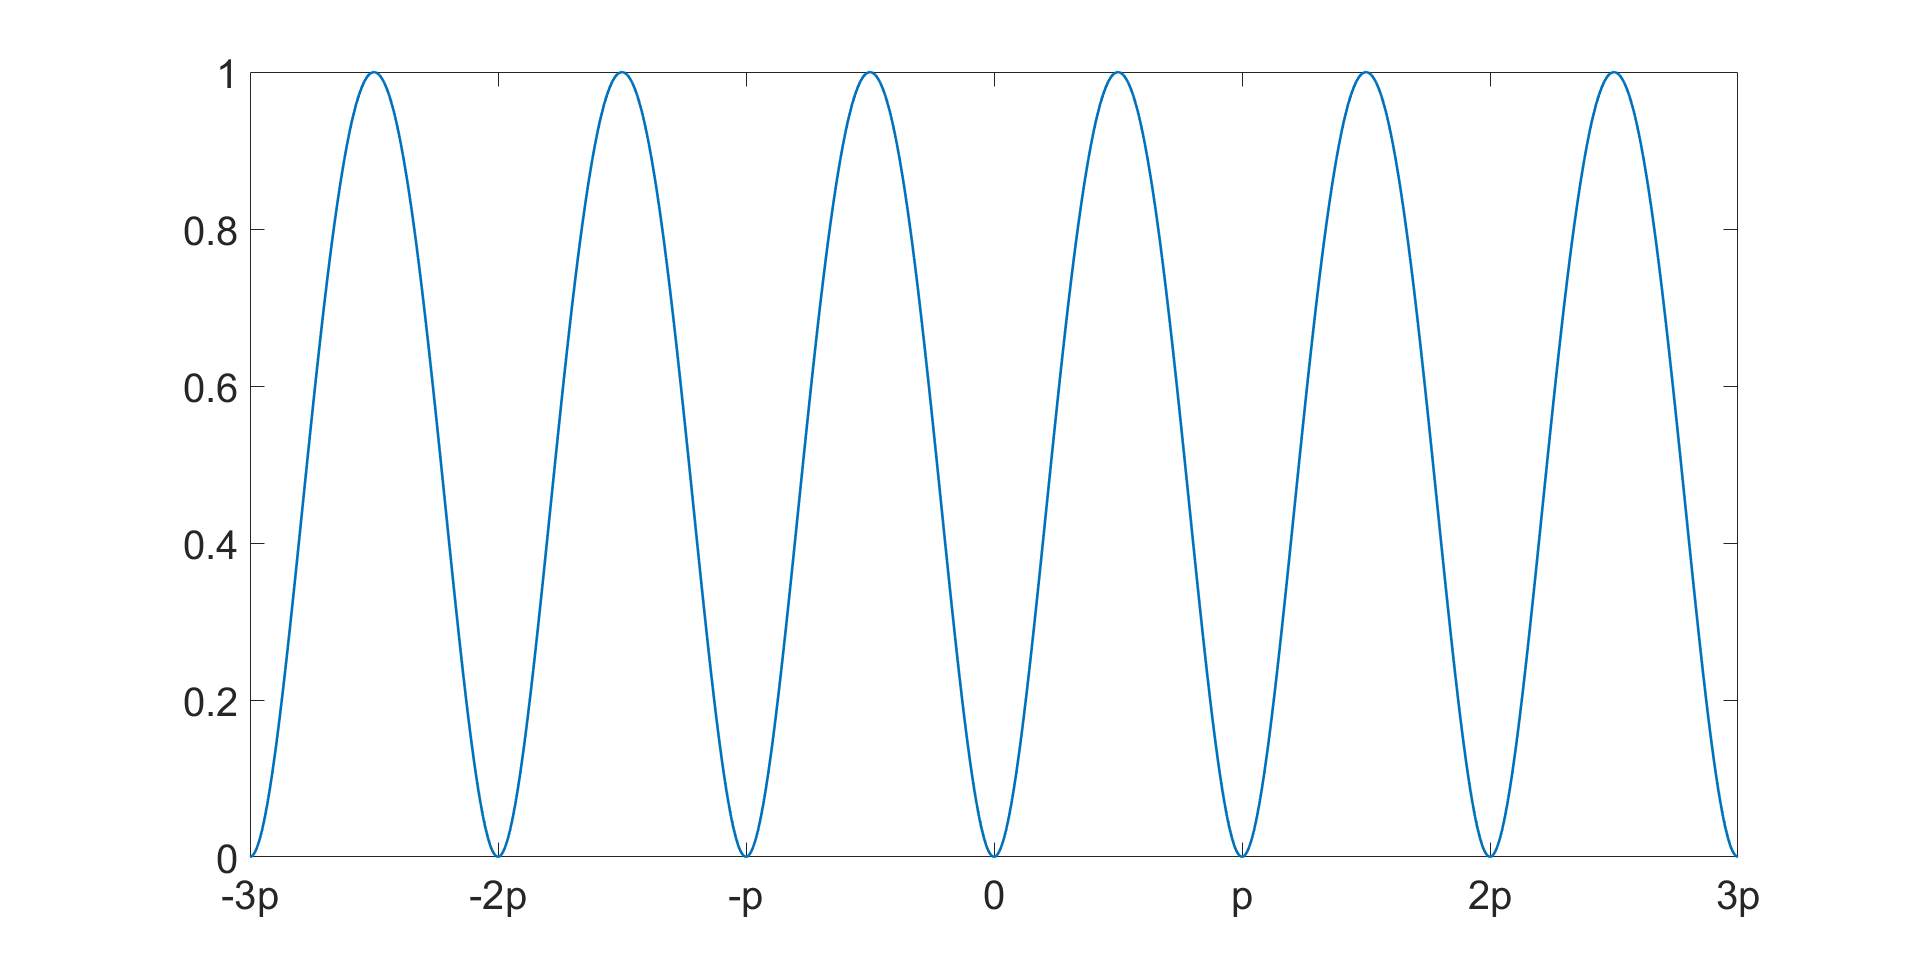
\includegraphics[width=12cm]{figures/periodic_function.png}
\caption[Polynomial Periodic Function]{A plot of $f_p\left(x\right)$ in the interval $\left[-3p, 3p\right]$. As can be seen, $f_p\left(x\right)$ is a priodic function, where its roots are equally spaced with a distance $p$.}
\label{fig:polynomial_periodic_function}
\end{figure}
\chapter{Gradient and Hessian Derivations}
In this appendix, we show detailed derivations for the gradient and Hessian of each individual penalty function, as defined in chapter \ref{chapter:method}.
\section{Angle Penalty Function}
The angle penalty functions is given by:
\begin{equation}\label{eq:angle_penalty}
\begin{split}
P_{\mathrm{angle}}\left(e_i,e_j\right) = \mathrm{sin} \bigg( 4\Big(\theta\left(e_i\right) - \theta\left(e_j\right)\Big) - \frac{\pi}{2}\bigg) + 1
\end{split}
\end{equation}
Where $\theta\left(e_k\right) = \mathrm{atan2}\Big(\mathrm{y}\left(v_k^2\right) - \mathrm{y}\left(v_k^1\right), \mathrm{x}\left(v_k^2\right) - \mathrm{x}\left(v_k^1\right)\Big)$ is the angle formed by half-edge $e_k = \left(v^1_k, v^2_k\right)$ with the positive \emph{x-axis} direction, when treated as a vector based at $v_k^1$ and heading $v_k^2$, for $k \in \left\{i,j\right\}$.

\noindent By denoting:
\begin{equation}\label{eq:angle_penalty}
x = \Big(\mathrm{y}\left(v_i^2\right), \mathrm{y}\left(v_i^1\right), \mathrm{x}\left(v_i^2\right), \mathrm{x}\left(v_i^1\right), \mathrm{y}\left(v_j^2\right), \mathrm{y}\left(v_j^1\right), \mathrm{x}\left(v_j^2\right), \mathrm{x}\left(v_j^1\right)\Big)^T
\end{equation}
And by replacing the sine expression with a polynomial periodic function $f_p$ with period $p=\frac{\pi}{2}$, as defined in appendix \ref{appendix:a}, we can rewrite $P_{\mathrm{angle}}$ as follows:
\begin{equation}\label{eq:angle_penalty_rephrased}
\begin{split}
P_{\mathrm{angle}}\left(x\right) = f_{\frac{\pi}{2}} \bigg(\alpha\left(x\right) - \beta\left(x\right)\bigg)
\end{split}
\end{equation}
Where $\alpha\left(x\right) = \mathrm{atan2}\Big(x_0 - x_1, x_2 -x_3\Big)$ and $\beta\left(x\right) = \mathrm{atan2}\Big(x_4 - x_5, x_6 -x_7\Big)$.
Its differential is given by:
\begin{equation}\label{eq:angle_penalty_rephrased_gradient}
\begin{split}
dP_{\mathrm{angle}}\left(x\right) = d\Bigg(f_{\frac{\pi}{2}} \bigg( \alpha\left(x\right) - \beta\left(x\right) \bigg)\Bigg)\\
 = f'_{\frac{\pi}{2}} \bigg(\mathrm{atan2}\Big(x_0 - x_1, x_2 -x_3\Big) - \mathrm{atan2}\Big(x_4 - x_5, x_6 -x_7\Big)\bigg)
\end{split}
\end{equation}